\documentclass[a4paper,12pt]{article}

% to make pdf searchable
\usepackage{cmap}

\usepackage{indentfirst}
\usepackage{fancyhdr}
\usepackage[T1,T2A]{fontenc}

% кодировка utf8, русские правила переносов
\usepackage[utf8]{inputenc}
\usepackage[russian]{babel}
\usepackage{amsmath}

% настраиваем поля
\usepackage[left=2cm,right=2cm,top=3cm,bottom=2cm]{geometry}

\usepackage{graphicx}
\usepackage{hyperref}
\usepackage{bookmark}
\usepackage[compact]{titlesec}

%\graphicspath{{\noiseimages}}
%\usepackage{graphicx}

\headheight16pt

% Даты исправлять только здесь
\newcommand{\olympdatestart}{1~ноября}
\newcommand{\olympyearstart}{2015}

\newcommand{\olympdateend}{1~декабря}
\newcommand{\olympyearend}{2016}

\newcommand{\olympcheckend}{20~января}

\newcommand{\olympmail}{fizleshcontest@yandex.ru}
%\newcommand{\olympmail}{contest@fizlesh.ru}

%\newcommand{\olympspocmail}{\href{mailto:demarin@mail.ru}{demarin@mail.ru}}
\newcommand{\olympspocmail}{\href{mailto:lilienberg@rambler.ru}{lilienberg@rambler.ru}}
%\newcommand{\olympspocphone}{\textbf{+7(910)473-69-06} (Дмитрий)}
\newcommand{\olympspocphone}{\textbf{+7(985)111-21-15} (Иван)}


\pagestyle{fancy}
\fancyhead{}
\fancyhead[LO]{Межрегиональная физическая олимпиада \olympyearstart---\olympyearend. Заочный тур}
\fancyhead[RO]{Стр.~\thepage~из 3}
\fancyfoot{}
\fancyfoot[RO]{\olympversion}

\newcommand\hr[1]{\left({#1}\right)}
\newcommand\un[1]{\,\emph{#1}}

\def\thesection{\arabic{section}.}
\def\thesubsection{\arabic{section}.\arabic{subsection}.}

\newcommand{\ctxitems}[1]{%
\begin{enumerate}
\setlength{\itemsep}{-3pt}
#1
\end{enumerate}}

\begin{document}
\section{Теоретические задачи}

В этой части части предлагается
дать максимально точный ответ, учтя наибольшее количество факторов, играющих роль в~каждой
задаче и~проявив знание необходимых законов физики.

\subsection{Прочность склейки}
Школьник Мстислав склеил торцы двух половинок доски клеем и~положил получившуюся конструкцию
горизонтально краями на опоры. Мстислав знает, что прочность клея на отрыв составляет 10~\emph{МПа}.
Какую массу груза Мстислав сможет поставить на место склейки так, чтобы конструкция не сломалась?
Как зависит ответ от размеров доски?

\subsection{Упругая деформация проволоки}
Школьник Радомир изучает упругие деформации твёрдых тел. У него есть график зависимости силы
натяжения проволоки от её удлинения для трёх видов проволоки из~одинакового металла, но
разной толщины (\emph{рис}.~1). Радомир хочет найти работу, затраченную на растяжение проволоки
средней толщины (сечением 1~\emph{мм}${}^2$) длиной $0.5$~\emph{м}
от~недеформированного состояния до~разрыва. Помогите ему сделать это.

\medskip
\centerline{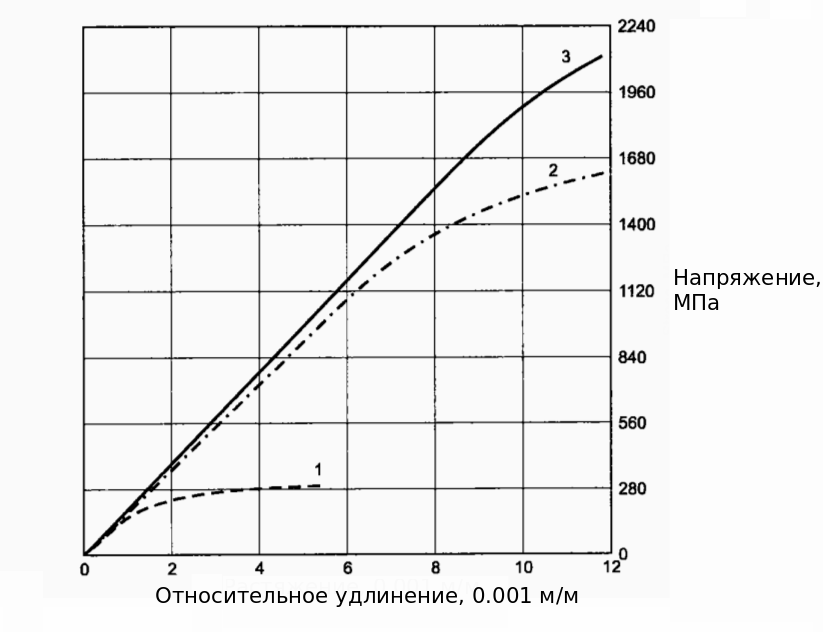
\includegraphics[height=60mm]{tension.png}}
\medskip
\centerline{\small Рис.~1}

\subsection{Свежий воздух}
Школьник Ярополк проветривает свою комнату. Он интересуется, как влияет на эффективность процесса
размер и расположение окна, температура и влажность наружного воздуха, а также скорость ветра.
Подумайте, как будет зависеть эффективность проветривания от этих факторов?
Что ещё будет влиять на неё?

\subsection{Загадочный цилиндр}
В своём кабинете физики школьник Изяслав обнаружил необычный цилиндр.
Изяслав положил его на наклонную плоскость. Вместо того, чтобы скатиться вниз,
цилиндр совершил пол-оборота вверх по плоскости и остановился.
Как бы вы объяснили это явление?

\subsection{Мир без сил}
Школьник Всеволод изучает силы поверхностного натяжения. Он размышляет о том, что было бы,
если бы этих сил в мире не существовало. А как вы думаете, как бы выглядел наш мир,
если бы в нём не было сил поверхностного натяжения?

\newpage

\section{Экспериментальные задачи}

Во этой части нужно проявить умение практического применения законов физики
и~проверки моделей, а~также умение грамотно интерпретировать результаты
эксперимента. Важно, что необходимо провести именно реальный,
а~не~мысленный эксперимент.

\subsection{Сладкая жизнь}
Добавляя сахар в стакан с водой, школьник Брячислав думает, как бы ему определить,
сколько сахара содержится в этом стакане. Помогите Брячиславу сделать прибор, позволяющий
определить концентрацию сахара в воде.

\subsection{Прочность <<гармошки>>}
Школьник Любомысл сложил лист бумаги <<гармошкой>>. Он хочет определить, насколько б\emph{о}льший
груз выдерживает такой лист, положенный двумя краями на опору, по~сравнению с~обычным.
Присоединитесь к исследованию Любомысла и~проверьте это экспериментально.

\subsection{Скорость дождя}
Глядя на идущий за окном дождь, школьник Лучезар думает, с какой скоростью падают капли дождя.
Как вы думаете, как Лучезар может измерить её экспериментально?

\subsection{Ёмкость батарейки}
Школьник Тихомир хочет померить ёмкость имеющихся у него батареек. Предложите способ,
которым он может это сделать, и проверьте его на~имеющихся у~вас батарейках.
Как результаты измерений будут зависеть от~нагрузки?

\subsection{Сопротивление слова}
Школьник Гостомысл, вертя в руке карандаш, думает о~том, как измерить электрическое
сопротивление написанного карандашом на бумаге слова <<олимпиада>> (слово написано
одним росчерком, не~отрывая карандаша от бумаги). Помогите ему сделать это.
В~решении укажите толщину линии.

\newpage

\section*{Краткие правила оформления работ}

\footnotesize

На титульном листе работы должно быть аккуратно написано:
\ctxitems{
\item Фамилия, имя, отчество участника олимпиады (полностью, печатными буквами)
\item Фамилии, имена, отчества родителей (полностью)
\item Школа, класс
\item Домашний адрес полностью, с индексом, названием населённого пункта и региона
\item Контактный телефон
\item Действующий адрес электронной почты (нужен для оповещения о приглашении на второй тур)
\item Название детского объединения (кружок, клуб) по физике, которое посещаете,\\
Ф.И.О. руководителей (полностью, печатными буквами)
\item Фамилия, имя, отчество учителя физики (полностью, печатными буквами)
}

Решать все задачи не обязательно. Лучше максимально полно ответить на вопросы задач,
рассмотреть интересные случаи. Возможно несколько решений, базирующихся
на разных идеях.

Можно пользоваться литературой и~другими источниками информации (Интернетом).
Работа выполняется индивидуально, \textbf{пользоваться помощью сверстников и учителей не разрешается}.

\input formatting

\bigskip
\normalsize

Удачи Вам!

\end{document}
